\documentclass[hyperref]{labbook}
\usepackage{verbatim}
\usepackage{graphicx}
\usepackage{hyperref}
\usepackage[a4paper,top=2cm,bottom=2cm,right=3cm,left=3cm]{geometry}
\usepackage[T1]{fontenc}
\usepackage{

\author{Jarvist Moore Frost}
\date{Jan 5th, 2010}

\begin{document}

\labday{6-1-11}

\experiment{PCBM-CG}

Continuuing the Girifalco CG C60 simulation work, the idea is to supplement the
single point forcefield by an interaction site to 'kinda' represent PBM.

This is done by defining a couple of atomtypes --- the C60 is standard Girifalco:
\begin{verbatim}
[ atomtypes ]
;type    mass    charge       ptype          sigma      epsilon
 C60    720.60   0.00           A           0.89535      26.822830
 PBM    190.00   0.00           A           0.5          10.0
\end{verbatim}

You then connect these things together with 'bonds' to specify their location,
and build up the bis / tris by specifying angles between the sidechains to
preserve the correct structure.

\subexperiment{Pymol Rendering}

Overlapping the two representations, and drawing spheres at the vdW radii (hard
sphere approximation) of the two coarse grain atoms, you get something a little
like this:

% F*R*E*C*K
%On Thu Jan  6 09:33:46 GMT 2011 in /home/jarvist/gmx_work/PCBM-CG/render_showing_CG_tris
%File: scene3.* became /home/jarvist/REPOSITORY/LABBOOK/PCBM-CG/figs/tris-CG-render.*
\begin{figure}[h!]
\centering
\includegraphics[width=0.8\columnwidth]{./figs/tris-CG-render.png}
\caption{\label{tris-CG-render}
Render of atomistic EEE Tris with superimposed vdW radii balls with the same parameters as the FF (well, the fullerene one might be off by 10\%, think this is the old incorrect reading of the Girifalco force field)
}
\end{figure}

In Pymol, going from the output PDB files, which open as orange and green blobs, you want to:

\begin{verbatim}
show spherse, all
alter elem P, vdw=2.5
alter elem C, vdw=4.47675
rebuild
\end{verbatim}

All together, with 10 mono PCBM on a wall, this looks something like:

% F*R*E*C*K
%On Thu Jan  6 10:10:48 GMT 2011 in /home/jarvist/gmx_work/PCBM-CG/monoPCBM_redo
%File: 10_mono_PCBM_stuck_on_wall.* became /home/jarvist/REPOSITORY/LABBOOK/PCBM-CG/figs/10_mono_PCBM_stuck_on_wall.*
\begin{figure}[h!]
\centering
\includegraphics[width=0.8\columnwidth]{./figs/10_mono_PCBM_stuck_on_wall}
\caption{\label{10_mono_PCBM_stuck_on_wall}
10 mono PCBM of the new build forecfield, with a dense wall of C60 sites below
them. MD at 300K, just to show behaviour and packing arrangement.  }
\end{figure}

\subexperiment{Parameterisation}

So, we basically have three free parameters with this paramterisation: Strength
of 'PBM' LJ potential, eqm distance of PBM LJ potential, and size of bond for
fullere---PBM.

LJ potentials are combined by geometric average of the $r^6$ and $r^{12}$
parameters (multiply them together + then sqrt) [type 1], or by the Lorentz-Beerthelot
rules (arithmetic avg for $\sigma$, geometric for $\epsilon$) [type 2]. 
But one can also
define the pairs explicitly in gromacs.

I guess what we really want to do is make use of the atomistic monoPCBM
forcefield, and fit the 3 parameters to reproduce similar CoM RDFs between the
CG representation and the atomistic. That should get the distances correct, ish, at least.

\subexperiment{RDFs}

So let's see how they compare currently...

\subexperiment{CG-RDF}

So make an index with 'a C' to 'make\_ndx -f confout.gro'.

And it looks quite interesting, you see the clear C60-C60 peak at just over
1nm, and then a 2nd peak which I imagine is from fullerene-fullerene with a PBM
stuck in the way. Perhaps. This is C60-C60 centre distance don't forget, no
contri from PBM:C60 or PBM:PBM.

% F*R*E*C*K
%On Thu Jan  6 10:44:26 GMT 2011 in /home/jarvist/gmx_work/PCBM-CG/monoPCBM_redo
%File: rdf.* became /home/jarvist/REPOSITORY/LABBOOK/PCBM-CG/figs/CG-RDF-early_work.*
\begin{figure}[h!]
\centering
\includegraphics[width=0.8\columnwidth,angle=270]{./figs/CG-RDF-early_work}
\caption{\label{CG-RDF-early_work}
Just a little simulation, 10 CG monoPCBM on a sticky wall. More or less
arbitrary guess parameters.  Lots of issues with this data---more of less
squashed on 2D wall, only a couple of neighbours at most etc. Need to do a
proper 3D volume simulation...
}
\end{figure}

\subexperiment{3D CG sim}

So the FF with the three variables are: $\sigma=$ 0.5, $\epsilon=$ 10.0, bond = 0.5

Looks like:
% F*R*E*C*K
%On Thu Jan  6 11:06:09 GMT 2011 in /home/jarvist/gmx_work/PCBM-CG/monoPCBM_redo
%File: monoPCBM-CG_1000_in_10x10x10_box_starting.* became /home/jarvist/REPOSITORY/LABBOOK/PCBM-CG/figs/monoPCBM-CG_1000_in_10x10x10_box_starting.*
\begin{figure}[h!]
\centering
\includegraphics[width=0.8\columnwidth]{./figs/monoPCBM-CG_1000_in_10x10x10_box_starting}
\caption{\label{monoPCBM-CG_1000_in_10x10x10_box_starting}
Starting configuration (after steepest descents relax) for 1000 CG monoPCBM in 10x10x10 box.
}
\end{figure}

And running under MD, it looks like:

% F*R*E*C*K
%On Thu Jan  6 11:12:14 GMT 2011 in /media/oldroot/home/jarvist/gmx_work/PCBM-CG/monoPCBM_redo
%File: monoPCBM-CG_1000_ngmx_render.* became /home/jarvist/REPOSITORY/LABBOOK/PCBM-CG/figs/monoPCBM-CG_1000_ngmx_render.*
\begin{figure}[h!]
\centering
\includegraphics[width=0.8\columnwidth]{./figs/monoPCBM-CG_1000_ngmx_render}
\caption{\label{monoPCBM-CG_1000_ngmx_render}
Nothing to do while running MD, so thought I'd capture a picture of the sim running in ngmx. Look like little fishies.
}
\end{figure}

Ok, did 10ns of MD, the RDF is now:

% F*R*E*C*K
%On Thu Jan  6 13:11:06 GMT 2011 in /media/oldroot/home/jarvist/gmx_work/PCBM-CG/monoPCBM_redo
%File: monoPCBM-CG_1000_rdf_10ns.* became /home/jarvist/REPOSITORY/LABBOOK/PCBM-CG/figs/monoPCBM-CG_1000_rdf_10ns.*
\begin{figure}[h!]
\centering
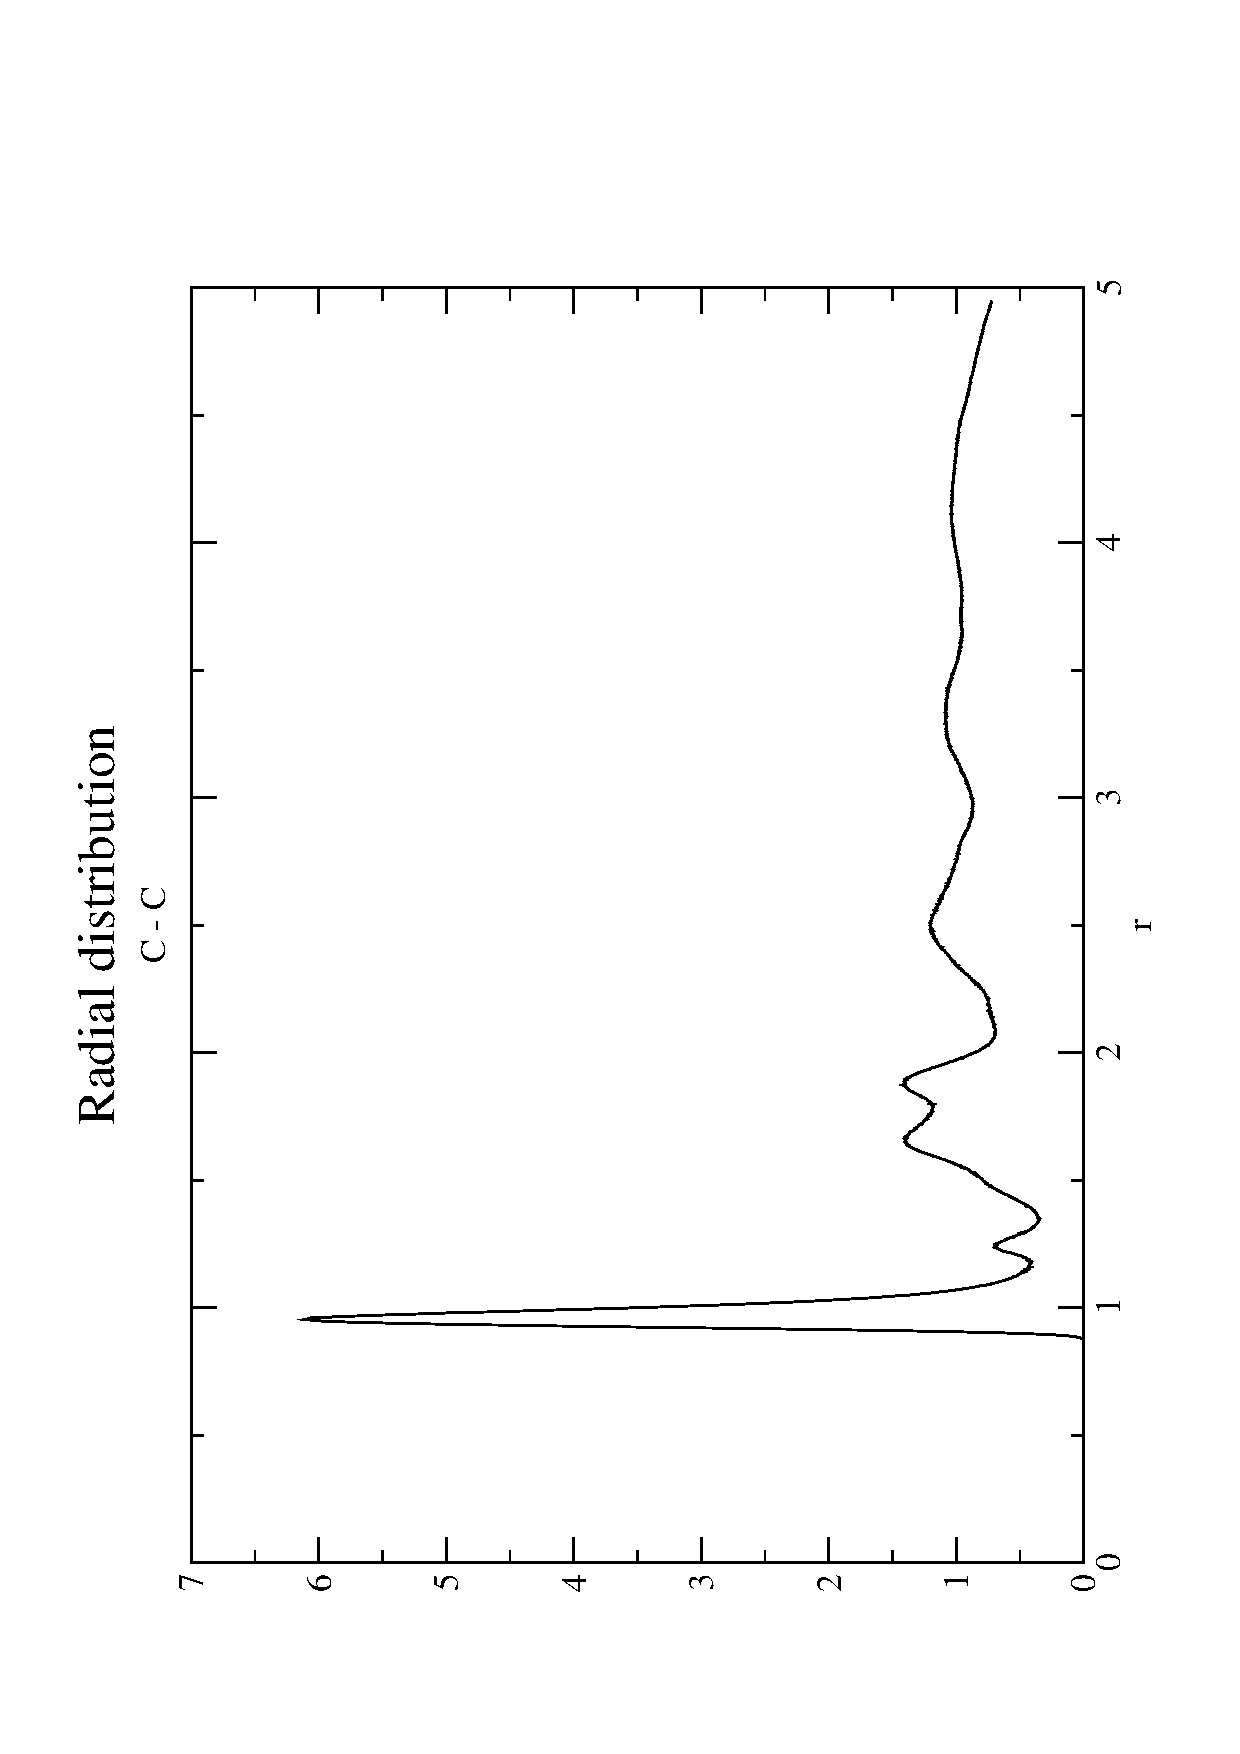
\includegraphics[width=0.8\columnwidth,angle=270]{./figs/monoPCBM-CG_1000_rdf_10ns}
\caption{\label{monoPCBM-CG_1000_rdf_10ns}
1000 mono PCBM CG force field, first stab... rdf from C60 sites - C60 sites, 10ns MD run with barostat + thermostat @ STP
}
\end{figure}

Just realised I'd be in remiss if I didn't do equiv. for a pure C60 simulation. Rather than reuse the stuff with Joe, I may as well restart a job from exact same initial conditions as this one...

\subexperiment{Initial monoPCBM vs. C60 Girifalco}

% F*R*E*C*K
%On Thu Jan  6 13:45:21 GMT 2011 in /media/oldroot/home/jarvist/gmx_work/PCBM-CG/monoPCBM_redo/C60_check
%File: monoPCBM-CG_1000_C60_vs_mono.* became /home/jarvist/REPOSITORY/LABBOOK/PCBM-CG/figs/monoPCBM-CG_1000_C60_vs_mono.*
\begin{figure}[h!]
\centering
\includegraphics[width=0.8\columnwidth,angle=270]{./figs/monoPCBM-CG_1000_C60_vs_mono}
\caption{\label{monoPCBM-CG_1000_C60_vs_mono}
5ns of C60 Girifalco vs. 10ns of monoPCBM first param.. Same starting conditions, barostat 1 atm, thermo 300K.
}
\end{figure}

\subexperiment{Compare to Atomistic...}

Hmm, bit challenging --- need to build index files.

PCBM has 88 atoms (therefore, 60 C60, 28 PBM).

Awk script to make index for C60 looked like:
\begin{verbatim}
BEGIN{
  for (i=0;i<99;i++)
     for (a=1;a<61;a++)
         print i*88+a
}
{}

for PBM:
BEGIN{
  for (i=0;i<99;i++)
     for (a=1;a<=28;a++)
         print 60+i*88+a
}
{}
\end{verbatim}

% F*R*E*C*K
%On Thu Jan  6 15:32:40 GMT 2011 in /home/jarvist/gmx_work/PCBM-CG/monoPCBM_redo/atomistic_relaxed_mono
%File: atomistic_mono_cg_rdfs.* became /home/jarvist/REPOSITORY/LABBOOK/PCBM-CG/figs/atomistic_mono_cg_rdfs.*
\begin{figure}[h!]
\centering
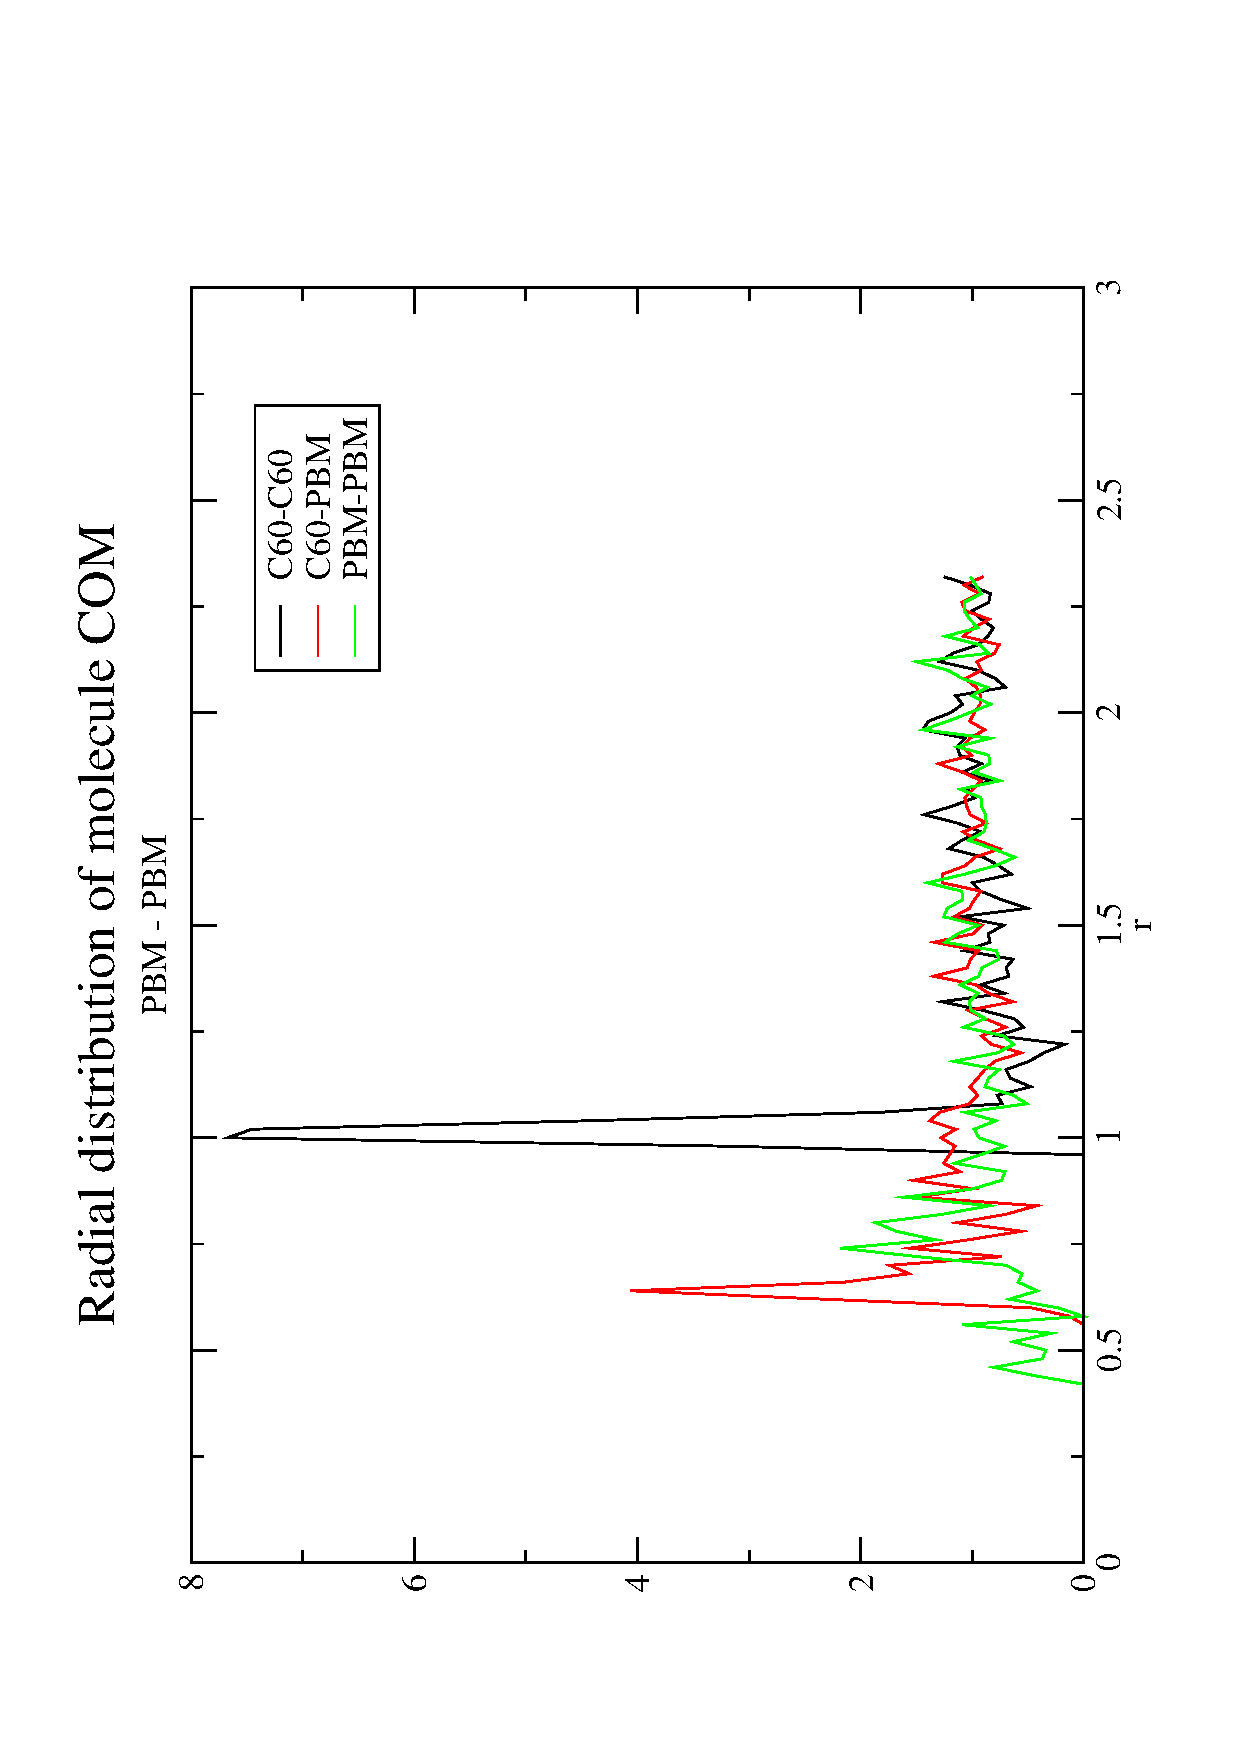
\includegraphics[width=0.8\columnwidth,angle=270]{./figs/atomistic_mono_cg_rdfs}
\caption{\label{atomistic_mono_cg_rdfs}
From a single frame of a 99-PCBM atomistic simulation, then steepest descents relaxation. Indexes composed with awk script, centre of mass molecular RDF for the components.
}
\end{figure}

And so now we go back to the CG simulations and reproduce the same:

% F*R*E*C*K
%On Thu Jan  6 15:43:29 GMT 2011 in /home/jarvist/gmx_work/PCBM-CG/monoPCBM_redo
%File: mono_CG_sims_CPC_rdf_comparison.* became /home/jarvist/REPOSITORY/LABBOOK/PCBM-CG/figs/mono_CG_sims_CPC_rdf_comparison.*
\begin{figure}[h!]
\centering
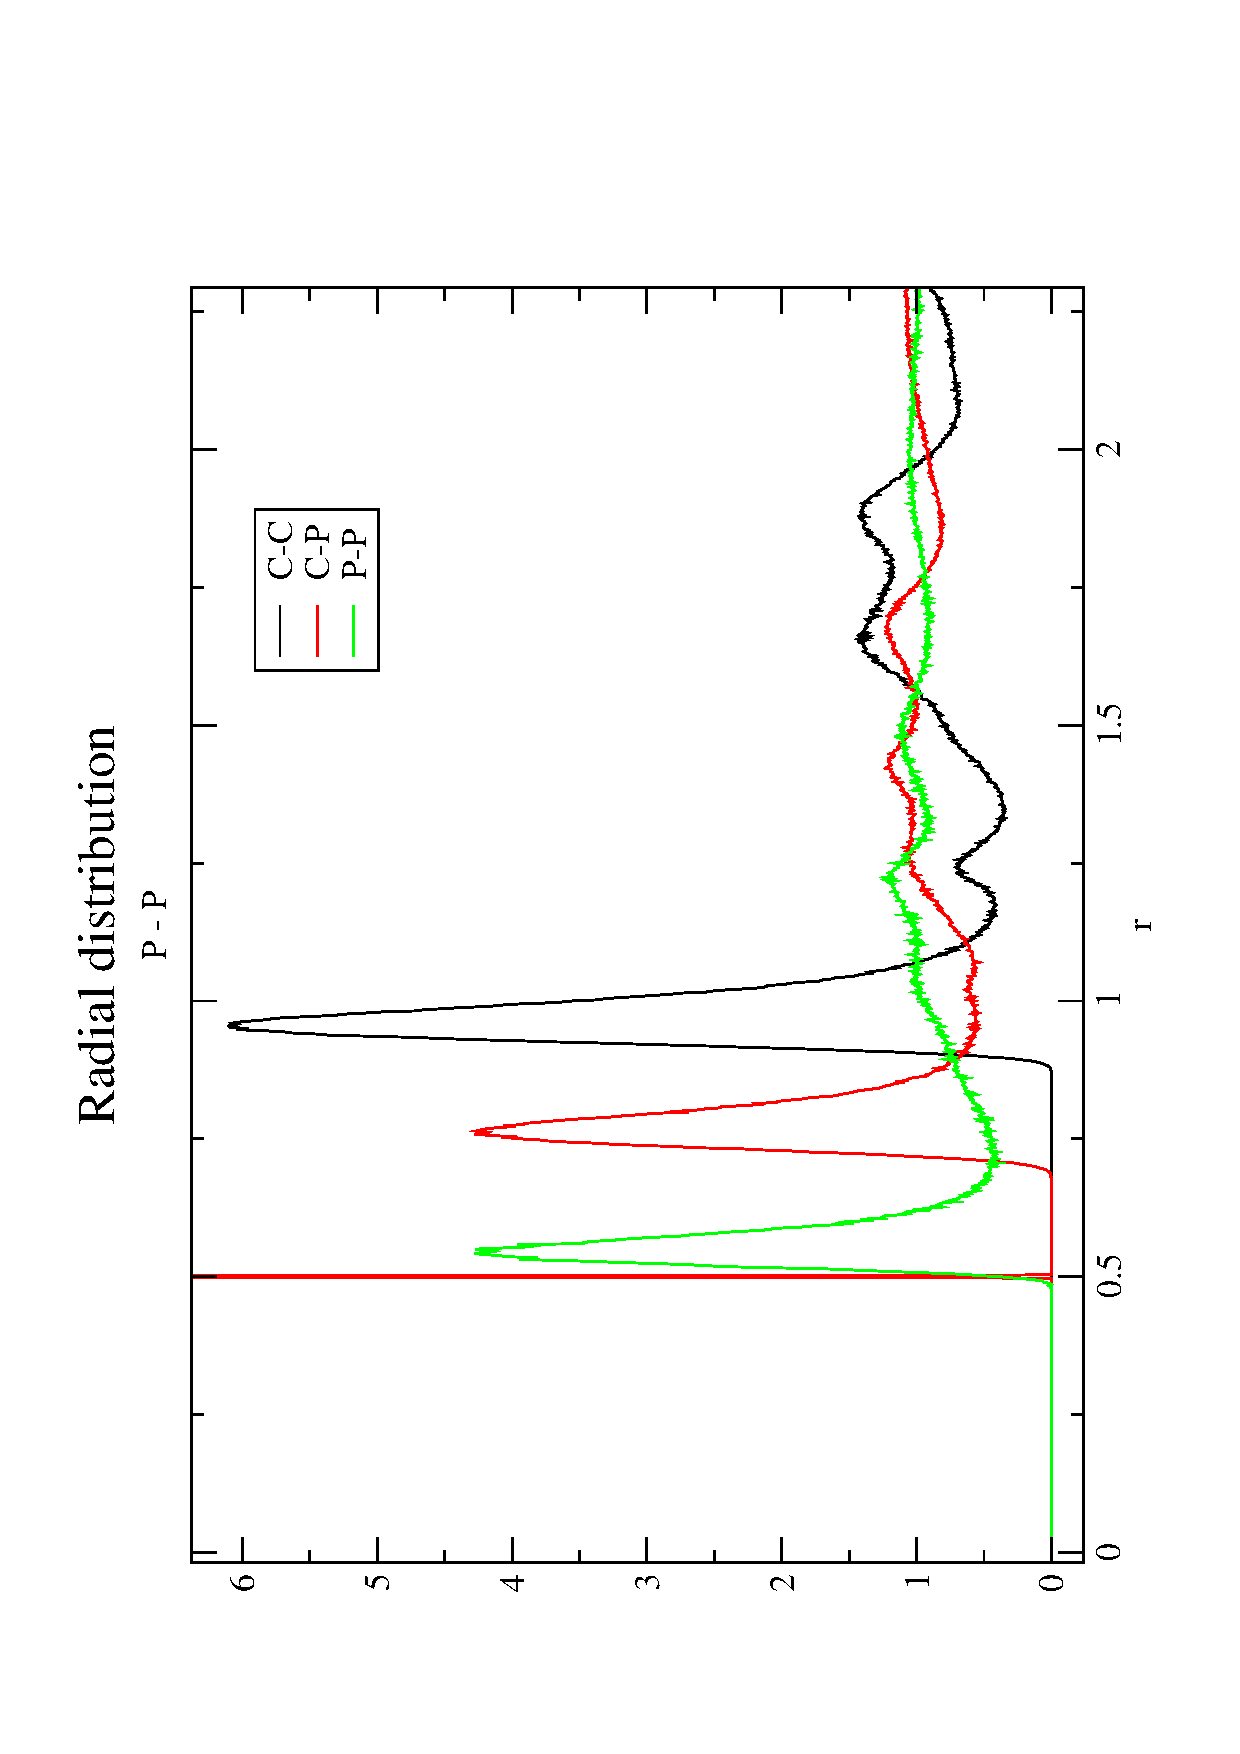
\includegraphics[width=0.8\columnwidth,angle=270]{./figs/mono_CG_sims_CPC_rdf_comparison}
\caption{\label{mono_CG_sims_CPC_rdf_comparison}
Comparison for the atomistic simulations, RDF from the 10ns early CG mono PCBM run, showing distances between the P(BM) + C(60) units, and amongst themselves. Note the large peak for the bonded part of the PCBM.
}
\end{figure}

\labday{7-1-11}

\subexperiment{Single monoPCBM-atomistic}

To check whether the RDFs included within single molecule contributions, I
looked at the C--C, C--P, P--P distances for a single PCBM from the atomistic
simulation (with -rdf mol\_com, and building an index with 1--60, 61--88).

This gave null results for C--C and P--P (as expected), and a value of 6.34 \AA
for C--P, which is a sample of the 'bonded' length between the C60 and PBM (CoM) on a single molecule.

% F*R*E*C*K
%On Fri Jan  7 14:31:15 GMT 2011 in /home/jarvist/gmx_work/PCBM-CG/monoPCBM_redo/2564_PCBM_atomistic
%File: RDFs_2564_20ps_MD_atomistic_PCBM.* became /home/jarvist/REPOSITORY/LABBOOK/PCBM-CG/figs/RDFs_2564_20ps_MD_atomistic_PCBM.*
\begin{figure}[h!]
\centering
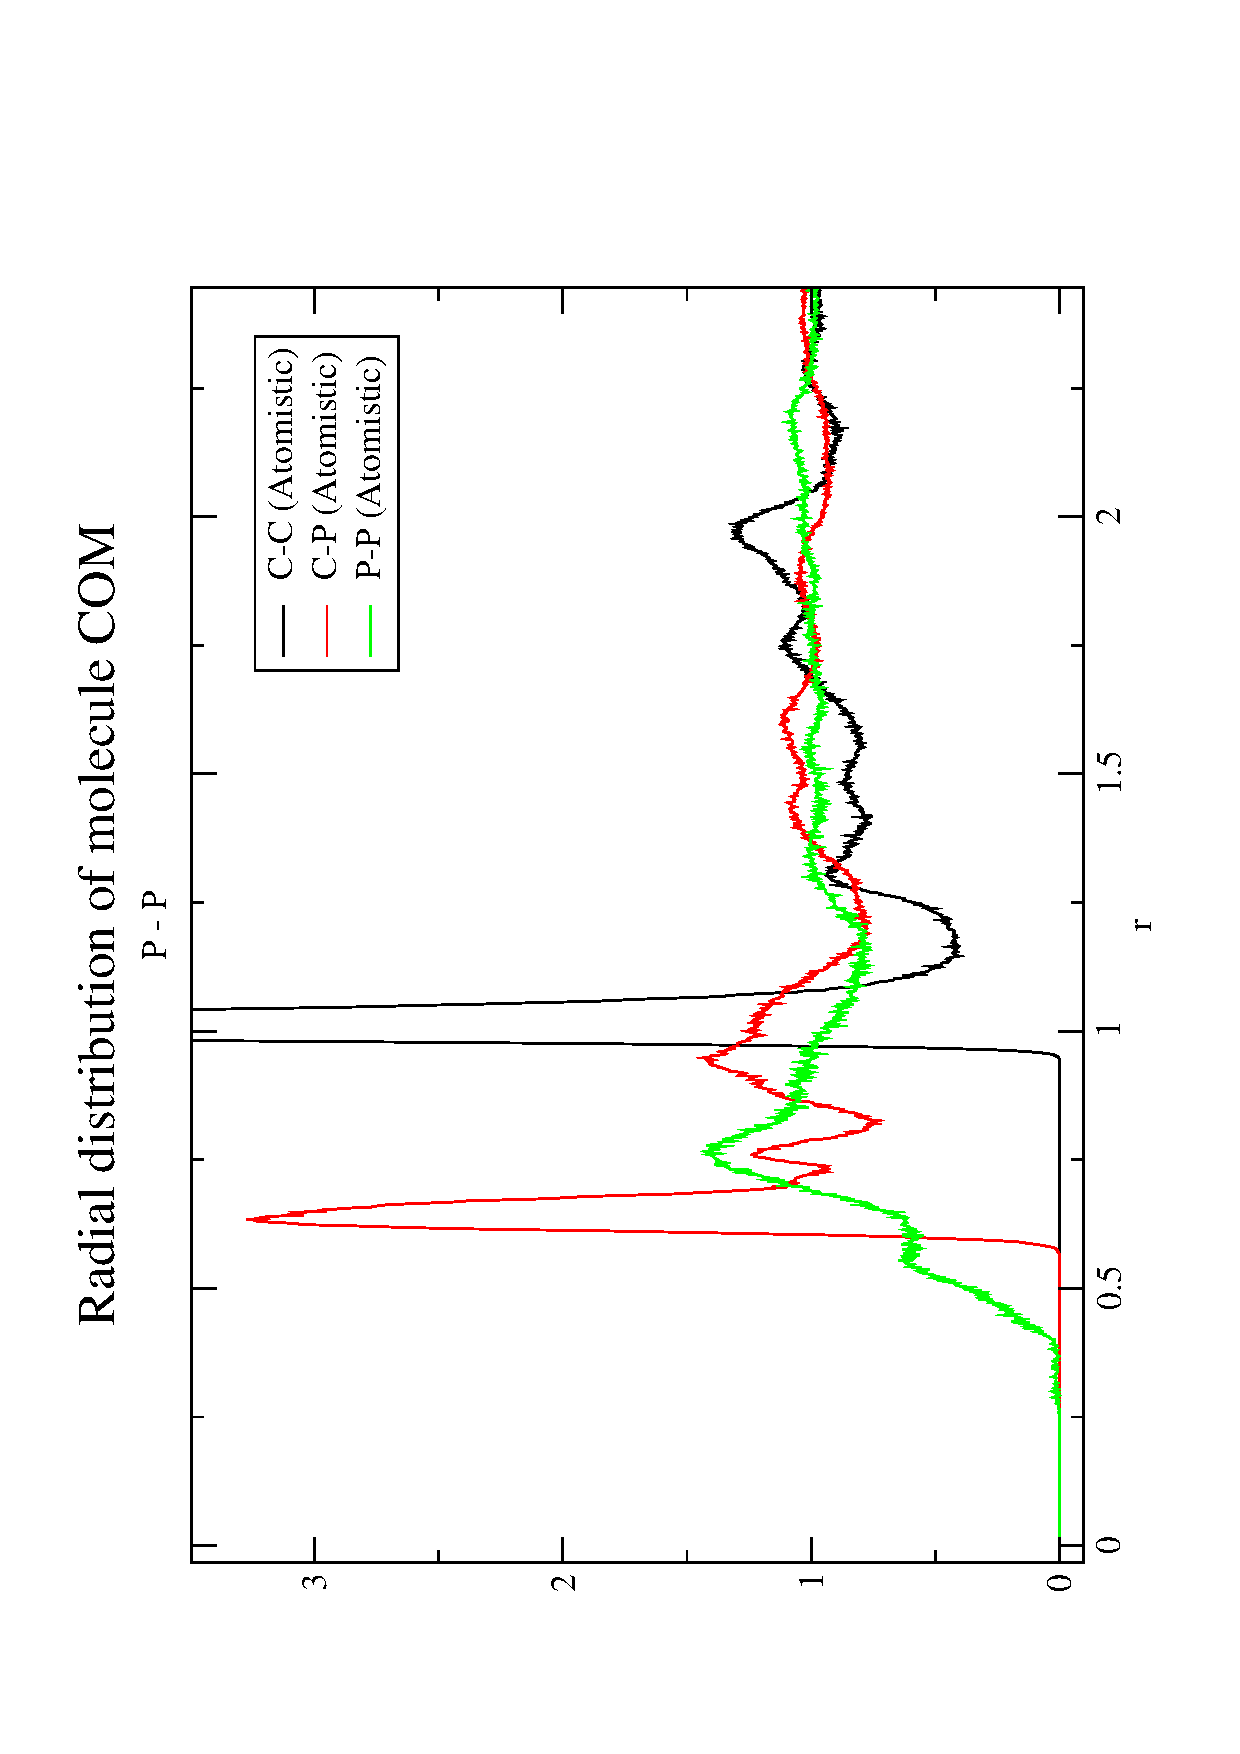
\includegraphics[width=0.8\columnwidth]{./figs/RDFs_2564_20ps_MD_atomistic_PCBM}
\caption{\label{RDFs_2564_20ps_MD_atomistic_PCBM}
Better (!) RDFs from a 2564 MD simulation I did a while ago, 20ps / 100 frames of data. Probably a better basis for the CG reconstruction.
}
\end{figure}

In the above assembly RDF, the C--P shortest distance has a strong peak at 6.34
\AA. There's a second bump around 7.6 \AA, perhaps this could be the
inter-molecular C60-PBM closest approach?



\end{document}
